\documentclass[fleqn]{jsarticle}

\usepackage{graphicx}
\usepackage{amsmath,amssymb}
\usepackage{amsmath}
\usepackage{fancyhdr}

\pagestyle{fancy}
\fancyhead[RE,RO]{先端データ解析論 レポート}

\usepackage{xcolor}
\usepackage[justification=centering]{caption}
\usepackage{listings}
\renewcommand{\lstlistingname}{リスト}
\lstset{language=Python,%
        % basicstyle=\footnotesize,%
        basicstyle=\tiny,%
        commentstyle=\textit,%
        classoffset=1,%
        keywordstyle=\bfseries,%
      	frame=tRBl,framesep=5pt,%
      	showstringspaces=false,%
        linewidth=35em,
      	}%

\begin{document}

\newcommand{\argmax}{\mathop{\rm argmax}\limits}

\title{先端データ解析論 第3回レポート}
\author{電子情報学専攻 48-176403 石毛真修}
\maketitle



\section*{大問1.}
$\argmax_{z} T(z) = \max(0, \theta + u - \lambda) + \min(0, \theta + u + \lambda)$
を証明する。

\subsubsection*{証明}
$T(z) = \lambda |z| + u (\theta - z) + \frac{1}{2}$ であるので、これを最大化するzは\\
$z \geq 0$ ならば、
\begin{eqnarray*}
  \frac{d}{dx} T(z) &=& \lambda - u - (\theta - z) = \lambda - u - \theta + z = 0\\
  \therefore z &=& \theta + u - \lambda
\end{eqnarray*}

$z < 0$ ならば、
\begin{eqnarray*}
  \frac{d}{dx} T(z) &=& - \lambda - u - (\theta - z) = - \lambda - u - \theta + z = 0\\
  \therefore z &=& \theta + u + \lambda
\end{eqnarray*}

よって、
\begin{eqnarray*}
  \argmax_{z} T(z) &=& \begin{cases}
    \theta + u + \lambda &(z < 0)\\
    \theta + u - \lambda &(z \geq 0)\\
  \end{cases}\\
  &=& max(0, \theta + u - \lambda) + min(0, \theta + u + \lambda)\\
\end{eqnarray*}







\section*{大問2.}
% \begin{figure}[h]
%   \begin{center}
%     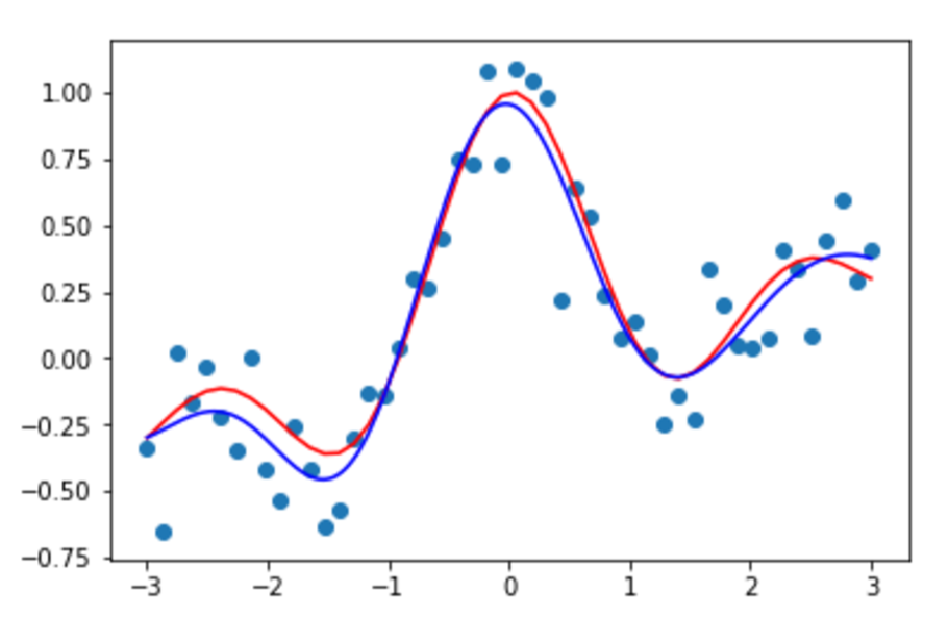
\includegraphics[width=0.6\textwidth]{figs/kernel_redge_basic.eps}
%   \end{center}
%   \caption{曲線 $y=\frac{sin(\pi x)}{\pi x} + 0.1x$ (赤)と $\lambda=0.1$, $h=0.7$ のときの回帰曲線(青).}
% \end{figure}


\begin{center}
\begin{tabular}{c}
  \begin{lstlisting}[]
    import matplotlib.pyplot as plt
    import numpy as np

    def org_model(x):
        return np.sin(np.pi * x) / (np.pi * x) + 0.1 * x

    def get_samples(x_samples, f):
        return f(x_samples) + 0.2* np.random.randn(len(x_samples))

    def kern(x, c, h=0.2):
        norm = x - c
        return np.exp(- norm**2 / (2 * (h**2)))

    kerns = np.vectorize(kern)
    def kern_matrix(x_samples, h=0.2):
        return np.array([kerns(xi, x_samples, h) for xi in x_samples])

    def ADM(samples_x, samples_y, lamb=1, h=0.2):
        dim = len(samples_x)
        u, z = np.zeros(dim), np.zeros(dim)
        K = kern_matrix(samples_x, h)

        iteration_cycles = 1500
        for i in range(iteration_cycles):
                theta = next_theta(K, samples_y, u, z, lamb, h)
                z = next_z(theta, u, lamb)
                u = next_u(theta, u, z)
        return theta

    def next_theta(K, y, u, z, lamb=1, h=0.2):
        Kt = np.transpose(K)
        Q = np.linalg.inv(np.matmul(Kt, K) + np.eye(len(y)))
        gamma = np.matmul(Kt, y) + z - u
        return np.matmul(Q, gamma)

    def next_z(theta, u, lamb=1):
        term1 = np.maximum(0, theta + u - lamb * np.ones(len(u)))
        term2 = np.maximum(0, - theta - u - lamb * np.ones(len(u)))
        return term1 - term2

    def next_u(theta, u, z):
        return theta + u - z

    def kern_model_gen(x_samples, y_samples, lamb=1, h=0.2):
        est_theta = ADM(x_samples, y_samples, lamb, h)
        def _model(x):
            return np.dot(est_theta, kerns(x, x_samples, h))
        v_model = np.vectorize(_model)
        return v_model


    np.random.seed()
    x_min, x_max = -3, 3
    n = 50
    N = 1000
    x = np.linspace(x_min, x_max, n)
    X = np.linspace(x_min, x_max, N)

    y = org_model(x)
    _y = get_samples(x, org_model)

    lamb = 0.1
    h = 0.7
    est_model = kern_model_gen(x, _y, lamb, h)
    Y = est_model(X)

    plt.scatter(x, _y)
    plt.plot(x, y, 'r-', X, Y, 'b-')
    plt.show()
  \end{lstlisting}
\end{tabular}{c}
\end{center}


\begin{figure}[h]
  \begin{center}
    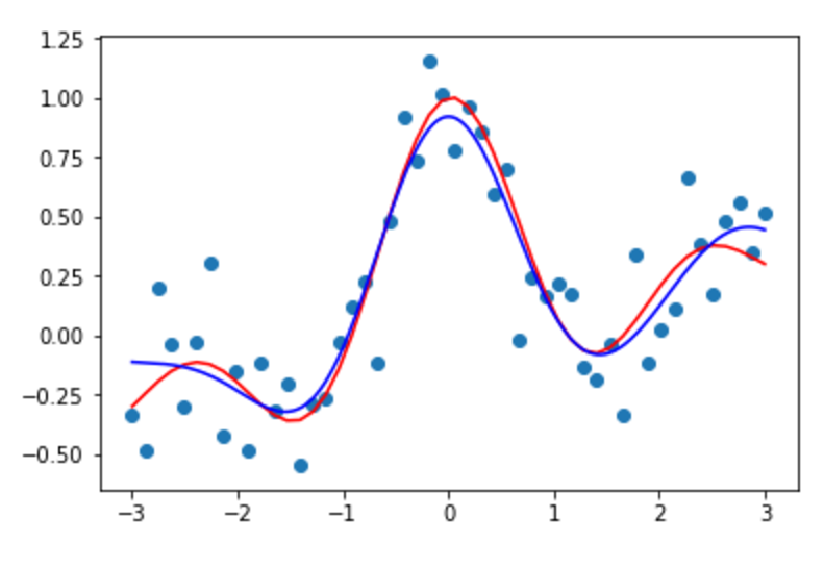
\includegraphics[width=0.8\textwidth]{figs/sparse_regression.eps}
  \end{center}
  \caption{スパース回帰の結果}
\end{figure}


\end{document}
